% THIS IS SIGPROC-SP.TEX - VERSION 3.1
% WORKS WITH V3.2SP OF ACM_PROC_ARTICLE-SP.CLS
% APRIL 2009
\documentclass{acm_proc_article-sp}
\usepackage[utf8]{inputenc}
\usepackage[english]{babel}
\usepackage{minted}
\usepackage{lineno}
\usepackage{hyperref}
\usepackage{enumitem}
\usepackage{amsmath}
\usepackage{tikz}
\usepackage{caption}
\usepackage{subcaption}
\usepackage{epigraph}
\usepackage{multirow}

%\usepackage{todonotes}
%\usepackage{marginnote} 
%\let\marginpar\marginnote

\usetikzlibrary{automata,arrows,positioning,calc,fit}
\linenumbers

\newcommand{\thesistitle}{Debugging Data-Flows in Reactive Programs}

\begin{document}

\title{\thesistitle}
%\subtitle{[Extended Abstract]}

\numberofauthors{3}
\author{
\alignauthor
Herman Banken\\
       \affaddr{Delft University of Technology, The Netherlands}\\
       \email{hermanb@ch.tudelft.nl}
\alignauthor
Georgios Gousios\\
       \affaddr{Delft University of Technology, The Netherlands}\\
       \email{g.gousios@tudelft.nl}
\alignauthor
Erik Meijer\\
       \affaddr{Delft University of Technology, The Netherlands}\\
       \email{h.j.m.meijer@tudelft.nl}
}

\date{\today} %10 Juli 2017}

\begin{minipage}[t][0.99\textheight]{0.99\textwidth}
%\begin{titlepage}
    \begin{center}
        \vspace*{1cm}
        
        \Huge
        \textbf{Visualizing Data-Flows \\in Reactive Programs}
        
        \large
		\vspace{0.5cm}
		by
        \vspace{0.5cm}
        
        \Large
        \textbf{Herman Banken}\\
		\normalsize
        born in Woerden, The Netherlands
        
        \vspace{1cm}
        \vfill

		to obtain the degree of Master of Science\\
		at the Delft University of Technology,\\
		to be defended publicly on Wednesday July 5th, 2017 at 4:00 PM.
        
        \vspace{0.8cm}
                
		\begin{tabular}{l l l}
		Student number:     & \multicolumn{2}{l}{4078624} \\
		Project duration:   & \multicolumn{2}{l}{September 10, 2016 - June 30, 2017} \\
		Thesis committee:   & Prof. Dr. H.J.M. Meijer, 	& TU Delft \\
    						& Dr. G. Gousios,           & TU Delft \\
    						& Prof. Dr. A van Deursen,  & TU Delft \\
    						& Joost de Vries,           & Ordina
		\end{tabular}

        \vspace{0.8cm}

		An electronic version of this thesis is available at \url{http://repository.tudelft.nl}.

\begin{minipage}{6in}
  \centering
  $\vcenter{\hbox{
\includegraphics[width=0.4\textwidth]{images/logo.png}}}$
  \hspace*{.2in}
  $\vcenter{\hbox{\includegraphics[width=0.4\textwidth]{images/ordina.png}}}$
\end{minipage}
        
    \end{center}
%\end{titlepage}
\end{minipage}

\maketitle
\begin{abstract}
\documentclass[11pt,a4paper]{article}
\usepackage{graphicx}
\usepackage{url}
\usepackage{hyperref}
\usepackage[top=1.25in, bottom=1.25in, left=1.25in, right=1.25in]{geometry}

\hypersetup{ colorlinks=true, linkcolor=cyan, filecolor=cyan,
urlcolor=cyan, citecolor=cyan, } \urlstyle{same}

\def\sectionautorefname{section}

\begin{document}

\title{ Thesis Proposal \\
Visualizing Data-Flows in Reactive Programs }
\author{ Herman Banken - 4078624
\vspace{1cm} \\
TU Delft, Department of Electrical Engineering, \\
Mathematics and Computer Science }
\date{\today}

\vfill

\begin{figure}[!bp]
    \centering
    \begin{minipage}[b]
        {0.4\textwidth} \includegraphics[width=\textwidth,trim={0 12cm 0
        10cm 0},clip]{images/tudelft.pdf}
    \end{minipage}
    \hfill
    \begin{minipage}[b]
        {0.4\textwidth} \includegraphics[width=\textwidth]{images/ordina.png}
    \end{minipage}
\end{figure}

\maketitle

\clearpage

\newcommand{\code}[1]{\texttt{#1}}

\section{Introduction}
general outline and research questions

problems with comprehension \& debugging in Reactive Programming \\
in recent Rx Contributor Days, paper Guido, experience

\begin{enumerate}
	\item[RQ1] How do developers comprehend and debug RP?
	\begin{enumerate}
		\item[RQ1.1] What strategies do developers use to comprehend RP?
		\item[RQ1.2] What debug tools do developers use to comprehend \& debug RP?
		\item[RQ1.3] ? Do experienced developers debug RP faster?
	\end{enumerate}

	\item[RQ2] How can we design a tool that helps developers debug Rx?
	\begin{enumerate}
		\item[RQ2.1] Can run-time behavior be extracted such that it is appropriate input to a visualizer?
		\item[RQ2.2] Can Rx programs be represented as graphs?
		\item[RQ2.3] Can Marble Diagrams effectively convey structures containing more than 1 operator?
	\end{enumerate}
		
	\item{RQ3} Can specialized debuggers speed up comprehension \& debugging?
\end{enumerate}


{\color{red}rest of paper}

\bibliographystyle{unsrt}
\bibliographystyle{abbrv}
\bibliography{papers/references}

%Visualizing Data-Flows in Functional Programs
%http://doi.ieeecomputersociety.org/10.1109/SANER.2016.82
%
%Reactive Extensions, Microsoft
%https://msdn.microsoft.com/en-us/data/gg577609.aspx
%
%Platform independent Reactive Extensions documentation
%https://reactivex.io
%
%Marble Diagrams explained in Channel9 video, Microsoft
%https://channel9.msdn.com/blogs/j.van.gogh/reactive-extensions-api-in-depth-marble-diagrams-select--where
%
%QuickCheck
%http://www.cs.tufts.edu/~nr/cs257/archive/john-hughes/quick.pdf
%
%Dynamic Taint Tracking for Java with Phosphor
%https://mice.cs.columbia.edu/getTechreport.php?techreportID=1601
%
%Phosphor on Github
%https://github.com/Programming-Systems-Lab/phosphor

\end{document}

\end{abstract}

% A category with the (minimum) three required fields
%\category{H.4}{Information Systems Applications}{Miscellaneous}
%A category including the fourth, optional field follows...
%\category{D.2.8}{Software Engineering}{Metrics}[complexity measures, performance measures]

%\terms{Theory}

\keywords{reactive programming, debugging, visualization, program comprehension} % NOT required for Proceedings


% \documentclass{acm_proc_article-sp}
% \usepackage{graphicx}
% \usepackage{url}
% \usepackage{hyperref}
% \usepackage[top=1.25in, bottom=1.25in, left=1.25in, right=1.25in]{geometry}

% \hypersetup{ colorlinks=true, linkcolor=cyan, filecolor=cyan,
% urlcolor=cyan, citecolor=cyan, } \urlstyle{same}

% \def\sectionautorefname{section}

% \begin{document}

% \title{Visualizing Data-Flows in Reactive Programs}
% \author{ Herman Banken - 4078624
% \vspace{1cm} \\
% TU Delft, Department of Electrical Engineering, \\
% Mathematics and Computer Science }
% \date{\today}

% \vfill

% \begin{figure}[!bp]
%     \centering
%     \begin{minipage}[b]
%         {0.4\textwidth} \includegraphics[width=\textwidth,trim={0 12cm 0
%         10cm 0},clip]{images/tudelft.pdf}
%     \end{minipage}
%     \hfill
%     \begin{minipage}[b]
%         {0.4\textwidth} \includegraphics[width=\textwidth]{images/ordina.png}
%     \end{minipage}
% \end{figure}

% \maketitle

% \clearpage


\newcommand{\code}[1]{\texttt{#1}}
%\newenvironment{todo*}[1]{\textcolor{red}#1}{}
\newcommand{\todo}[1]{
\textcolor{red}{#1}
}
\newcommand{\todov}[1]{
{\color{red}
#1
}
}

% Stanford writing guide http://cs.stanford.edu/people/widom/paper-writing.html

\section{Introduction}
general outline and research questions

problems with comprehension \& debugging in Reactive Programming \\
in recent Rx Contributor Days, paper Guido, experience

\begin{enumerate}
	\item[RQ1] How do developers comprehend and debug RP?
	\begin{enumerate}
		\item[RQ1.1] What strategies do developers use to comprehend RP?
		\item[RQ1.2] What debug tools do developers use to comprehend \& debug RP?
		\item[RQ1.3] ? Do experienced developers debug RP faster?
	\end{enumerate}

	\item[RQ2] How can we design a tool that helps developers debug Rx?
	\begin{enumerate}
		\item[RQ2.1] Can run-time behavior be extracted such that it is appropriate input to a visualizer?
		\item[RQ2.2] Can Rx programs be represented as graphs?
		\item[RQ2.3] Can Marble Diagrams effectively convey structures containing more than 1 operator?
	\end{enumerate}
		
	\item{RQ3} Can specialized debuggers speed up comprehension \& debugging?
\end{enumerate}


\section{Background: RP}

\label{background}
\subsection{Reactive Programming}
\label{nutshell}
Reactive Programming (RP) is a declarative programming paradigm for working with streams of input data. 
According to the original definition\footnote{
``Reactive programs [..] maintain a continuous interaction with their environment, at a speed which is determined by the environment, not the program itself.''~\cite{berry1989real}
} a reactive program must interact with the environment `at a speed which is determined by the environment'.
This means that when a reactive program is run it sets up the data pipeline declared in the code and waits until input arrives c.q. the environment changes.
Reactive Programming languages and libraries provide developers with the appropriate abstractions and methods to create such programs.

The programming paradigm of Reactive Programming is implemented by multiple languages and libraries. Many RP implementations share a notion of a collection that abstracts over \textit{time}, in contrast to \textit{space} like standard collections, be it \textit{Observable} (Rx~\cite{meijer2010subject}), Signal (Elm~\cite{czaplicki2012elm}), Signal/Event (REScala~\cite{salvaneschi2014rescala}) or Behavior/Event (FRP~\cite{elliott1997functional}). In this paper we focus on the Rx formulation, but our work is applicable to other RP implementations to some extend. 

Understanding how we, given the Rx language, arrive at our visualization requires at least minimal understanding of Rx.
Rx introduces two types \textit{Observable} and \textit{Observer}, derived by dualizing the Iterable and Iterator types. Observables define the data flow and Observers receive the data, possibly moving the data further down the stream. Figure \ref{sample1} shows a very basic example of a in situ data flow in Rx. First an Observable is created, here using the static \code{of} method, then dependent Observables are created using the \code{map} and \code{filter} methods on the Observable instance. Finally we \code{subscribe} to start the data flow and send the data in the flow to the console (eg. JavaScript's stdout).

\begin{figure}

\begin{subfigure}[a]{\columnwidth}
\inputminted[tabsize=2]{javascript}{listings/sample1.js}	
\caption{Rx code example}
\label{sample1}
\end{subfigure}

\begin{subfigure}[b]{\columnwidth}
\centering
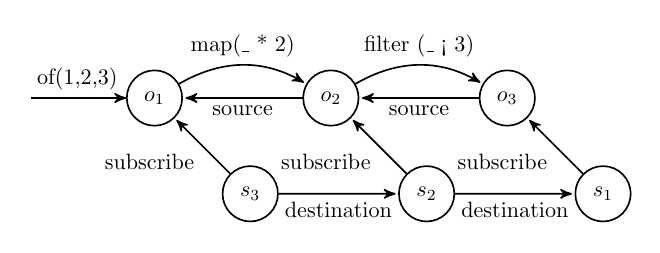
\begin{tikzpicture}[->,>=stealth',shorten >=1pt,auto,node
    distance=2.8cm,
                    semithick,scale=0.8, every node/.style={scale=0.8}]
    \tikzstyle{every state}=[]

    \node[state] (A) {$ o_1 $}; \node[state] (B) [right of=A] {$ o_2 $};
    \node[state] (C) [right of=B] {$ o_3 $};

    \node[state] (X) [below right =1cm of A] {$ s_3 $}; \node[state] (Y)
    [right of=X] {$ s_2 $}; \node[state] (Z) [right of=Y] {$ s_1 $};

    \path (B) edge node {source} (A) (C) edge node {source} (B) (A) edge
    [bend left] node {map(\_ * 2)} (B) (B) edge [bend left] node {filter
    (\_ < 3)} (C) (X) edge node[below] {destination} (Y) (Y) edge node[below]
    {destination} (Z) (Z) edge node {subscribe} (C) (Y) edge node {subscribe}
    (B) (X) edge node {subscribe} (A);

    \draw[<-] (A) -- node[above] {of(1,2,3)} ++(-2cm,0);
    %\draw[<-] (Z) -- node[below] {subscribe} ++(2cm,0);

\end{tikzpicture}

\caption{Rx graph example}
\label{chaincreate}
\end{subfigure}

\caption{Basic Rx  Observables}

\end{figure}

It is important to note that Observables are lazy, they are the blueprint of a data flow. Only when the \code{subscribe} method of Observable is called the data flow is created by recursively subscribing up the stream. \textit{Observer}s are subscribed to each Observable until the source Observables are reached which then are setup and can start emitting the data.
This is illustrated in figure \ref{chaincreate}. Here $o_1$, $o_2$ and $o_3$ represent Observables defined in Figure \ref{sample1}. Inside the \code{subscribe} call $s_1$ is created and passed to $o_3$, which in turn will recursively subscribe to $o_2$ with a new Observer $s_2$ with destination $s_1$, until the full chain is subscribed.
The origin of this design is the duality between Observables and \textit{Iterables} - as first described by Meijer~\cite{meijer2010subject}, where Observers are dual to \textit{Iterators}.

\begin{figure}

\begin{subfigure}[a]{\columnwidth}
\inputminted[tabsize=2]{javascript}{listings/sample3.js}	
\caption{Higher order flatMap operation}
\label{sample3}
\end{subfigure}

\begin{subfigure}[b]{\columnwidth}
\centering
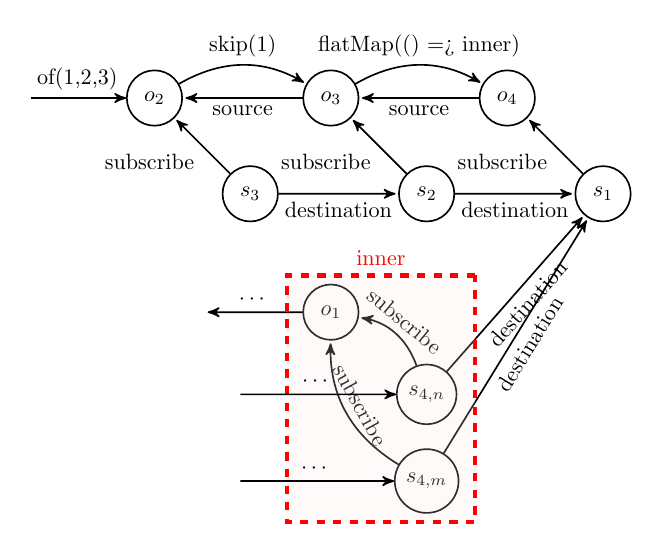
\begin{tikzpicture}[->,>=stealth',shorten >=1pt,auto,node
    distance=2.8cm,
                    semithick,scale=0.8, every node/.style={scale=0.8}]
    \tikzstyle{every state}=[]

    \node[state] (A) {$ o_2 $}; \node[state] (B) [right of=A] {$ o_3 $};
    \node[state] (C) [right of=B] {$ o_4 $};

    \node[state] (X) [below right =1cm of A] {$ s_3 $}; \node[state] (Y)
    [right of=X] {$ s_2 $}; \node[state] (Z) [right of=Y] {$ s_1 $};

    \node[state] (F) [below =2cm of B] {$ o_1 $}; \node[state] (P) [below
    =1.8cm of Y] {$ s_{4,n} $}; \node[state] (Q) [below =0.3cm of P] {$
    s_{4,m} $};

    \path (B) edge node {source} (A) (C) edge node {source} (B) (A) edge
    [bend left] node {skip(1)} (B) (B) edge [bend left] node {flatMap(()
    => inner)} (C) (X) edge node[below] {destination} (Y) (Y) edge node[below]
    {destination} (Z) (Z) edge node {subscribe} (C) (Y) edge node {subscribe}
    (B) (X) edge node {subscribe} (A)

    (P) edge [bend right] node[sloped,above] {subscribe} (F) (P) edge
    node[sloped,below] {destination} (Z) (Q) edge [bend left] node[sloped,above]
    {subscribe} (F) (Q) edge node[sloped,below] {destination} (Z);

    %  \node[draw=none] (K) at ($ (P) + (-4:-3) $){$\cdots$};
    %  \node[draw=none] (M) at ($ (Q) + (-4:-3) $){$\cdots$};

    % https://tex.stackexchange.com/questions/75497/automata-container-box
    \node [draw=red, label={\color{red}inner}, fit=(F) (P) (Q), inner
    sep=0.5cm,dashed, ultra thick, fill=red!10, fill opacity=0.2] {};
    %\node [draw=blue, fit= (G) (Q) (M), inner sep=0.5cm,dashed, ultra thick, fill=blue!10, fill opacity=0.2] {};

    % https://tex.stackexchange.com/questions/160643/ellipsis
    \draw[<-] (A) -- node[above] {of(1,2,3)} ++(-2cm,0); \draw[->] (F)
    -- node[above] {$ \cdots $} ++(-2cm,0); \draw[<-] (P) -- node[above]
    {$ \cdots $} ++(-3cm,0); \draw[<-] (Q) -- node[above] {$ \cdots $}
    ++(-3cm,0);

\end{tikzpicture}

\caption{Higher order visualization}
\label{chainhigher}
\end{subfigure}

\caption{Higher order Observables}

\end{figure}

More complex programs feature operators that merge Observables, split Observables or handles higher order Observables, resulting in more complex graphs. While merging and splitting happens on an Observable level (the \code{source} property still points to the dependency) higher order Observable flattening manifests only in Observer structure, as shown in Figure \ref{chainhigher}.

Creating the Observable we will call the \textit{assembly} phase, the phase where the subscribe happens the \textit{subscription} phase and data flows in the \textit{runtime} phase. The three phases can be interleaved for different streams, for example when dealing with higher order Observables,  meaning one could use Observables as values inside the data flow. The Observables used as values have yet to start the second phase while the outer stream is in the runtime phase.


\begin{figure}[t]
\centering
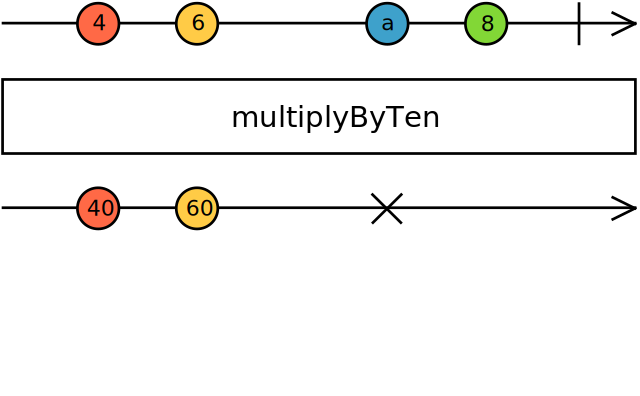
\includegraphics[width=\columnwidth]{images/marble-diagram.pdf}
\caption{Marble Diagram}
\label{marblediagram-image}
\end{figure}

\paragraph{Marble Diagram}
\label{marblediagram}
The term \textit{Marble Diagram} comes from the shape of the glyps in the images used to explain Rx in the official documentation. 
The diagrams contain one or more timelines containing the events that enter and leave Observables. 
Next-events are typically represented with a circle, an error-event with a cross and a complete-event with a vertical line.
Developers can see from the diagram how operators work by inspecting the difference between the timelines, 
where events might be skipped, added, transformed or delayed. 
Mapping time on the x-axis provides insight that is missing when inspecting only a single time slice. 

\section{Research Design}
To answer our research questions we employ a mixed methods research approach as shown in Table~\ref{research-methods}.
First we interview professional developers and review available documentation (RQ1) to form a understanding about current debugging practices,
then we apply this understanding to design a debugger and implement it to test its feasibility (RQ2),
finally we validate the debugger using an experiment (RQ3).

\begin{table}[t]
\centering
\begin{tabularx}{\columnwidth}{lllX}
\hline
\textbf{}            & \textbf{Method} & \textbf{Focus}                               \\ \hline
\multirow{2}{*}{RQ1} & Interview       & What are current practices                   \\ 
                     & Literature      & What is recommended                          \\
\multirow{2}{*}{RQ2} & Design          & What can a RP debugger show                  \\ 
                     & Implement       & Extract meta information from Rx             \\ 
RQ3                  & Experiment      & Quantification of effect on debugging        \\ \hline
\end{tabularx}
\caption{Research Methods used in the study}
\label{research-methods}
\end{table}

\iffalse
\todo{
qualitive data
quantitive
design, implemented, tested with real developers
buzz words: mixed methods, grounded theory
}
\fi

\section{RP Debugging practices}
\label{section-practices}

%\todo{alternative section titles: Evaluating motivation / collecting empirical evidence / case study}
To validate the need for better tools we must first understand what existing tools are used (RQ1).
We interview developers as we want to explore and understand the current practices, instead of using an experiment or survey to test a particular hypothesis.
A controlled experiment to verify some hypothesis formed from literature could fail to include any practices employed that we did not consider.
The questions were semi-structured. We first established a general understanding of the experience of the subjects.
Then we asked several open questions regarding use of RP, how subjects debug RP and test RP. Table \ref{interview-questions} lists the questions used a guideline for the interviews.

\begin{table*}[]
\centering
\caption{Interview questions}
\label{interview-questions}
\begin{tabular}{ll}
    & \textbf{Question}                                               \\ \hline
Q1  & Explain your (professional) experience.                         \\ \hline
Q2  & Assess your experience on a scale from beginner to expert.      \\ \hline
Q3  & Explain your (professional) reactive programming experience.    \\ \hline
Q4  & Assess your RP experience on a scale from beginner to expert.   \\ \hline
Q5  & Did you refactor or rework RP code?                             \\ \hline
Q6  & Did you and how did you test or verify the workings of RP code? \\ \hline
Q7  & Did you and how did you debug RP code?                          \\ \hline
Q8  & Did you and how did you use documentation on RP?                \\ \hline
Q9  & What difficulties did you experience with RP?                   \\ \hline
Q10 & What is your general approach to understand a piece of Rx?      \\ \hline
\end{tabular}
\end{table*}

Five developers with professional programming experience ranging from 4 to 12 years where interviewed. 
Those developers work in a company building mostly reactive systems~\footnote{\url{http://www.reactivemanifesto.org/}} using various RP solutions,
and range from personal experience to over a year of Rx experience.
Furthermore we interviewed one subject from our university with 4 years of occasional Rx experience.

\subsection{Interview results}
Of the 6 subjects only the subject without professional experience did not debug Rx. 
The other 5 subjects all independently mentioned using println-debugging in several forms (println, logging, console log).
One subject mentioned that while adding log statements is easy it required him to recompile the project which could take several minutes, 
which caused him to rely more on breakpoints using the Chrome debugger.
Another subject - which experience was mostly with RxScala - mentioned that he did not use breakpoints as those `are difficult to use with asynchronous computations'.
A third subject used the NodeJs debugger but describes using it as `painful' as he stepped through the inners of Rx.


\subsection{Literature and written work}
Developers can learn Rx through several sources such as the official documentation at \href{http://reactivex.io}{reactivex.io}, books, online courses and from the many blog posts available. The official documentation\footnote{
	\url{https://github.com/Reactive-Extensions/RxJS/blob/master/doc/gettingstarted/testing.md\#debugging-your-rx-application}
} mentions the use of the \code{do}-operator to add tracing to console. Five books we reviewed on different versions of Rx contained a debugging chapter with tips like adding the Rx version specific \code{do}-like operators~\cite{esposito2016reactive,rxjavabook2016} or do not have a debugging chapter at all~\cite{introtorx, rxjavabook2015, rxswiftbook2017}. Esposito and Ciceri~\cite{esposito2016reactive} further explain how to best format the log statements and introduce ways to limit the logging by modifying the Observable through means of throttling and sampling. The RxJava book~\cite{rxjavabook2016} also contains tips to use the various \code{do} operators to integrate with existing metric tools.
To our knowledge the only article addressing issues of debugging Rx is by Staltz, one of the contributors of RxJS\footnote{\url{http://staltz.com/how-to-debug-rxjs-code.html}}, noting that conventional debuggers are not suitable for the higher level of abstraction of Observables. Staltz explains three current ways to debug Rx, being (1) tracing to the console, (2) manually drawing the dependency graph, (3) manually drawing marble diagrams.

The available literature matches the results of the interviews. \code{printf}-debugging is commonly advised and used. While the conventional debugger works in some cases this is mostly for the procedural logic that interleaves Rx logic. Automated tooling is suggested, but is not implemented.  


\input{chapters/current}

\section{Debugger Design}
\label{section-design}
In this section we describe the design of a visualizer for the ReactiveX (Rx) family of RP libraries to answer RQ2. Given the findings of RQ1, the requirements for our visualizer are:
\begin{description}
\itemsep0em 
\item[REQ1] Provide overview of Observable flows
\item[REQ2] Provide detailed view inside flow
\end{description}

We propose a visualizer consisting of two parts: (1) a data flow graph and (2) a dynamic marble diagram. The data flow graph provides high-level overview, showing how different flows are created, combined and used, while the marble diagram offers a more in-depth look into a single selected data flow showing the contents (in terms of values and subscriptions) of the flows and can be used learn the behaviors and interplay of operators.

\subsection{Data Flow Graph}
\paragraph{Simplified graphs} When running an RP program, Observables are created that depend on other Observables (their \emph{source}) and Observers are created to send their values to a defined set of Observers (their \emph{destination}). Figure \ref{chaincreate} shows these relations in a graph. For the simplest of programs, the relations between the Observables ($O = {o_1, o_2, o_3}$) and those between Observers ($S = {s_1, s_2, s_3}$) share an equally shaped sub-graph after a reversal of the Observer-edges. To provide more overview, we process the graph to merge the two Observable and Observer sequences together, simplifying it in the process, as in Figure \ref{fiddlesimple}. Higher order relations are retained as shown in \ref{fiddlehigher}.

\begin{figure}[ht]
	\centering
	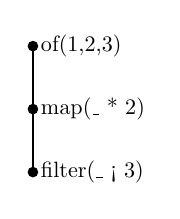
\begin{tikzpicture}[->,>=stealth',shorten >=1pt,auto,node distance=1.5cm,
                    semithick,scale=0.8, every node/.style={scale=0.8}]
\tikzstyle{every state}=[]
\filldraw 
  (0,2) circle (2pt) node[right] {of(1,2,3)} --
  (0,1) circle (2pt) node[right] {map(\_ * 2)}     -- 
  (0,0) circle (2pt) node[right] {filter(\_ < 3)};
\end{tikzpicture}

	\caption{Simplified graph of Figure \ref{chaincreate}}
	\label{fiddlesimple}
\end{figure}

\begin{figure}[ht]
	\centering
	
\begin{tikzpicture}[->,>=stealth',shorten >=1pt,auto,node
    distance=1.5cm,
                    semithick,scale=0.8, every node/.style={scale=0.8}]
    \tikzstyle{every state}=[] \filldraw (0,2) circle (2pt) node[right]
    {of(1,2,3)} -- (0,1) circle (2pt) node[right] {skip(1)} -- (0,0)
    circle (2pt) node[right] {flatMap(() => inner)};

    \filldraw (-1,1) circle (2pt) node[left] {of(`A', `B')} -- (0,0)
    circle (2pt) node[right] {};

    \filldraw (-0.7,1) circle (2pt) node[left] {} -- (0,0) circle (2pt)
    node[right] {};

\end{tikzpicture}

	\caption{Simplified graph of Figure \ref{chainhigher}}
	\label{fiddlehigher}
\end{figure}

\paragraph{Layout} Layout is used to add extra meaning to the graph. If multiple subscriptions on the same Observable are created, multiple flows are kept in the graph and they are bundled together in the resulting layout. This is designed to help developers find related flows. Also it is easy to see that for example an Observable is reused many times, hinting a possible performance improvement by sharing the computation (Rx has special \code{share}-operators to multicast). The layout is based on StoryFlow~\cite{liu2013storyflow}, which employs a hierarchical clustering before ordering the graph in a way to reduce crossings. Where StoryFlow clusters on physical character location we cluster flows per Observable. Furthermore, StoryFlow supports interactivity in various layout stages of which we use the algorithms for \emph{straightening} and \emph{dragging} to support selecting a specific flow, which is then highlighted, straightened and positioned at the right in order to match the marble diagram, shown for the current highlighted flow.

\paragraph{Color} Coloring the nodes can be used to identify the same Observable in multiple places in the graph, as Observables can be reused in different places of the stream.

\subsection{Dynamic Marble Diagrams}
In contrast to the original diagrams (Section \ref{marblediagram}) we use dynamic diagrams which update live when new events occur and are stacked to show the data in the complete flow. This allows the developer to trace a value back through the flow, a debug operation which is impossible using a classic debugger. Handcrafted marble diagrams can use custom shapes and colors to represent events, but for the generic debugger we use only three shapes: next-events are a green dot, errors a black cross, completes a vertical line, as shown in Figure~\ref{screenshot-mergeAll}. For our generic debugger it is unfeasible to automatically decide which properties (content, shape and color) to apply to events, as the amount of events and distinguishing features might be unbounded. Instead the event values are shown upon hovering.

\subsection{Architecture}
To support the visualization, we design a debugger architecture consisting of 2 components:

The \textbf{Host instrumentation} instruments the Rx library to emit useful execution events. Depending on the language and platform, specific instrumentation is required. Output of the instrumentation is a platform and language independent graph like Figure \ref{chainhigher}. By splitting the instrumentation, the debugger can be used for the complete ReactiveX family of libraries by only reimplementing the first component. The communication protocol for the instrumentation is shown in Table \ref{protocol}. 

The \textbf{Visualizer} takes the initial graph and simplifies it into a Data Flow Graph. Then it lays out the Data Flow Graph and provides the debuggers User Interface. By separating the visualizer, we can safely export generated graphs and visualize them post mortem for example for documentation purposes.

The components can run in their own environment. The instrumentation must run inside the host language, while the Visualizer can use a different language and platform.

\begin{figure*}
\includegraphics[width=\textwidth]{{images/screenshot.mergeAll.crop}.png}
\caption{Screenshot of \href{http://rxfiddle.net/\#type=editor&code=Y29uc3Qgc291cmNlMSA9IFJ4Lk9ic2VydmFibGUKICAub2YoMSwgMiwgMywgNCkKCmNvbnN0IHNvdXJjZTIgPSBSeC5PYnNlcnZhYmxlCiAgLm9mKCJhIiwgImIiLCAiYyIsICJkIikKClJ4Lk9ic2VydmFibGUKICAub2Yoc291cmNlMSwgc291cmNlMikKICAubWVyZ2VBbGwoKQogIC5za2lwKDIpCiAgLnN1YnNjcmliZSgp}{RxFiddle.net}}
\label{screenshot-mergeAll}
\end{figure*}

\begin{table*}[t]
\centering
\resizebox{\textwidth}{!}{%
\begin{tabular}{|l|l|}
\hline
addObservable(id, sourceIds)                   & Adds a Observable node, with zero or more source Observable's                                                                                                                      \\ \hline
addObserver(id, observableId, destinationId)   & \begin{tabular}[c]{@{}l@{}}Add a Observer, observableId denotes the Observable it subscribed to, \\ optional destinationId adds an edge to the destination Observer\end{tabular}   \\ \hline
addOuterObserver(observerId, outerDestination) & \begin{tabular}[c]{@{}l@{}}Create a special edge between an existing Observer and the higher order \\ destination Observer\end{tabular}                                            \\ \hline
addEvent(observerId, type, optionalValue)      & \begin{tabular}[c]{@{}l@{}}Add an event to the Observer denoted by observerId, of type (next, error, complete), \\ optionally with a value (for next / error events).\end{tabular} \\ \hline
addMeta(id, metadata)                          & Add meta data such as the method call which created an Observable.                                                                                                                 \\ \hline
\end{tabular}%
}
\caption{Instrumentation protocol}
\label{protocol}
\end{table*}

\subsection{Implementation}
To validate the design and to provide an implementation to the developer community we created \url{RxFiddle.net}. The RxFiddle project is a reference implementation of 
our reactive debugger design. Besides the visualizer, the website also contains a code editor for JavaScript code with sharing functionality, for developers to share snippets with their peers, as shown in Figure \ref{screenshot-mergeAll}. In this section we will explain different parts of the implementation. For RxFiddle, we initially focused on RxJS (JavaScript).

\paragraph{Instrumentation}
With JavaScript being a dynamic language, we use a combination of prototype patching and Proxies\footnote{\url{https://developer.mozilla.org/docs/Web/JavaScript/Reference/Global_Objects/Proxy}} to instrument the RxJS library: the Observable and Observer prototypes are patched to return Proxies wrapping the API method calls. The instrumentation passes every method entry and method exit to the Linking-step.

\paragraph{Linking}
Here, we distinguish between method calls from the different phases (Section \ref{nutshell}). From the assembly phase, we detect when Observables are used as target or arguments of a call or as return value, and create a graph node for each detected Observable. We add an edge between the call target \& call arguments and returned Observables, denoting the `source'-relation. Also, we tag the returned Observable with the call frame information (time, method name, arguments). In the subscription phase we detect calls to the \code{subscribe}-method: the destination Observers are passed as arguments, so we create the graph nodes and save the relation as an edge. In the runtime phase we detect `next', `error' and `complete' calls on Observers and add these as meta data to the Observer nodes.

\paragraph{Graph Loggers}
From the Linking-step the graph mutations are streamed to the environment of the visualizer, where the graph is rebuild. Depending on the host language a different protocol is used: RxFiddle's code editor executes the code in a Worker\footnote{\url{https://developer.mozilla.org/docs/Web/API/Worker}} and transmits events over the postMessage protocol, while RxFiddle for Node transmits over WebSockets. Being able to support multiple protocols increases the possible use cases, ranging from the code editor for small programs, to the Node plugin for server applications, to Chrome DevTool extensions\footnote{\url{https://developer.chrome.com/extensions/devtools}} for web applications.

\paragraph{Visualizer}
The visualizer receives the current state in the form of a graph from the Logger. It then uses the Observers in the graph to create the Data Flow Graph (DFG). 
To layout the DFG using StoryFlow~\cite{liu2013storyflow} we first rank the graph using depth first search, remove slack and reverse edges where necessary to create a directed acyclic graph. We then add dummy nodes to replaces long edges with edges spanning a single rank. Finally we order and align the nodes in the ranks assigning coordinates for the visualization. It is important that layout is fast, as it runs every time the DFG is changed. To render the Marble Diagrams the flow to and from the selected Observer is gathered by recursively traversing the graph in the direction of the edges, respectively the reversed direction.


\section{Evaluation}
In this section we evaluate our ideas about the debugger which we designed by answering RQ3. First we present the experiment that we designed, then explain the context in which we organized the experiment and finally we present the results.

\subsection{Object and Method}
The goal of the experiment is to measure the \textit{time} required to solve programming problems. We assume time is a measurement for ease of debugging. Participants use either the built-in Chrome debugger (group `Console') or - the treatment - our RxFiddle debugger (group `RxFiddle'). This single alternative debugger together with the experiment UI (which acts as a small IDE) offers all the debugging capabilities subject reported to use in our preliminary interviews.

The experiment consists of a questionnaire, a warm-up program and 4 programming problems, all available in a single in-browser application. The questionnaire contains questions regarding age, experience in several programming languages and several reactive programming frameworks. We use this self estimation as  a measurement of skill instead of a pretest, since it provides ~\cite{kleinschmager2011rate,feigenspan2012measuring,siegmund2014measuring}. The warm-up program is situated in the same environment as the programming problems and contains several tasks designed to let the participants use every control of the test environment. The first 2 programming problems require the participants to gain some knowledge about the behavior of the program and report the findings. The last 2 programming problems contain a program with a bug. The participants are asked to find the event that lead to the bug in the third problem and to identify and propose a solution in the fourth problem. The first 2 problems are synthetic examples of two simple data flows, while the latter contain some mocked (otherwise remote) service which behaves like a real world example.

We use a between-subjects design for our setup. While this complicates the results - subjects have different experience and skills - we can not use a within-subjects design as it would be impossible to control for the learning effect incurred when asking subjects to perform survey questions with and without the tool. This also allows us to restrict the amount of tasks to incorporate in the experiment, requiring less time of our busy subjects.

\todo{Discuss guidelines defined in ko2015practical~\cite{ko2015practical}}

\subsection{Context}
The experiment was run in a controlled and an online setting.
The controlled experiment was conducted at a Dutch software engineering company. Subjects are developers with several years of programming experience, and range from little to no experience with RP to many years of experience (Figure \ref{fig-experience}). Some of the subjects had already used RxFiddle, forming a potential threat to validity. As we do not try to measure the effect of learning a new tool, but rather using a tool after learning to use it, we explained RxFiddle in the introductory talk and added the warm-up question to get every participant to a minimum amount of knowledge about the debugger at hand.

The online experiment was announced by several core contributors to RP libraries on Twitter and via various other communication channels. Subjects to the online experiment took the test at their own preferred location and have possibly very different backgrounds. Several short video tutorials were created and included in the online experiment to introduce the participants to the debug tool available to them and the tasks they needed to fulfill.

\begin{figure}[h]
\includegraphics[width=\columnwidth]{images/experience.pdf}
\caption{Experience in various programming languages, 9-point Likert scale}
\label{fig-experience}
\end{figure}

\subsection{Results}
Figure \ref{fig-timePerTask} shows the time until the correct answer was given per task. Here we consider both the results from the controlled experiment as the online experiment, to remedy the small set of subjects available for the controlled experiment. We immediately see some interesting result for task 3. We do not know the underlying distribution so we perform a non-parametric Wilcoxon Mann-Whitney U test (\textit{$H_0$: times for the Console group and RxFiddle group are drawn from the same population}) to see if the differences are significant, and a Cliffs delta test for ordinal data to determine the effect size.

\begin{centering}
\begin{tabular}{llllll}
    \hline
                & \textbf{$n_1$} & \textbf{$n_2$} & \textbf{W} & \textbf{p-value} & \textbf{Cliff's $\delta$} \\
    \hline
    \textbf{T1} & 34             & 36             & 559        & 0.540            & 0.0866                   \\
    \textbf{T2} & 32             & 31             & 517        & 0.780            & -0.0424                  \\
    \textbf{T3} & 23             & 28             & 96         & $6.19e^{-6}$     & 0.702                    \\
    \textbf{T4} & 13             & 12             & 60         & 0.347            & 0.231                    \\
    \hline
\end{tabular}
\end{centering}

For tasks T3 we can reject $H_0$ with high significance ($p < 0.05$), the RxFiddle group is faster.
For the tasks T1, T2 and T4 we can not reject $H_0$ ($p > 0.05$), and for T2 the U test indicates no difference at all, meaning the RxFiddle group and Console group perform or could perform equally. While this could be observed as a negative result, RxFiddle is a new tool, and the users have only just been exposed to the tool and received only a short training. Of course it could also be the case  that RxFiddle might be more suitable to replace some tasks than others. From the results of the experiment we can not give a definitive explanation for the comparable results.

\begin{figure}[h]
\includegraphics[width=\columnwidth]{images/timePerTask.pdf}
\caption{Time until correct answer per task}
\label{fig-timePerTask}
\end{figure}


\subsection{Validity}
\textbf{Subjects.} The online experiment was open to anyone who wanted to participate. As a result a mixed group of developers took part, even those without Rx experience. The total amount of participants filling in the preliminary survey for the experiment was larger than the group finishing the experiment.

\textbf{Tasks.} The experiment consists of 2 small and 2 medium tasks, so the results of the experiment might not necessarily generalize to debugging RP in practice with larger systems. For larger tasks the effects of the debugger could be bigger and therefore be better measurable. Still we chose for these smaller tasks, for two reasons: in the limited time of the subjects they could answer only so many questions and designing larger tasks for the experiment would take many more iterations and time. With the limited amount of time available we still show that a significant speed-up can be achieved in some cases. We leave it for future work to extend the experiment to include larger systems.


\section{Discussion}
\subsection{Applicability}
The experiment consists of 2 small and 2 medium tasks, so the results of the experiment might not necessarily generalize to debugging RP in practice with larger systems. For larger tasks the effects of the debugger could be bigger and therefore be better measurable. Still we chose for these smaller tasks, for two reasons: in the limited time of the subjects they could answer only so many questions and designing larger tasks for the experiment would take many more iterations and time. With the limited amount of time available we still show that a significant speed-up can be achieved in some cases. We leave it for future work to extend the experiment to include larger systems.

\subsection{Scalability}
Debugging large reactive systems over longer periods of time can result in significantly larger Observable graphs and Marble Diagrams than currently evaluated. During tests of RxFiddle with larger applications like RxFiddle itself and an existing Angular application the graph became too large to render in a reasonable amount of time. Besides rendering performance, a potentially even bigger issue is with communicating large graphs to the developer. We propose several extensions to RxFiddle to remedy this issue: (1) pruning the graph of old flows to show only the active flows, (2) bundling flows that have the same structure and only rendering a single instance offering a picker into the flow of interest, (3) collapsing certain parts of the graph that are local to one source file or function, (4) adding search functionality to quickly identify flows by operator or data values, (5) support quick navigation between code \& graph.

Furthermore we think that while Marble Diagrams are useful for small to medium amount of events ($< 20$), both better performance and better functionality would be achieved by providing a different interface for high volume flows. Above a certain threshold of events this interface could be the default, offering features like filtering, watch expressions (to look deeper into the event's value), and advanced features like histograms \& FFT.

\subsection{Visualization}
Our implementation visualizes higher order flows as a combination of the original flow with incoming edges from the merged flows. While this visualization matches the behavior of merging streams together it does not map conceptually with some other use cases of higher order flows, for example using one Observable as stop condition for another Observable (\code{takeUntil}).

\subsection{Breakpoints}
Setting traditional breakpoints in a reactive program stops the system from being reactive, and therefore can change the behavior of the system. This was our reason not to deal with breakpoints in RxFiddle. However, the behavior of breakpoints is twofold: they allow us to modify the application state by interacting with the variables in scope, but they also provide a way to be notified of an event occurrence. While the first is arguably not desirable for reactive systems, the notification property might be a good addition to RxFiddle. BIGDEBUG~\cite{Gulzar2016}, a debugging solution for systems like Spark, introduces \textit{simulated breakpoints} for this purpose. When a simulated breakpoints hits the execution resumes immediately and the required lineage information of the breakpoint is collected in a new independent process. Implementing this for RxFiddle is a matter of creating the right UI as the required lineage data is already available.



\subsection{Limitations}
\paragraph{Graph scalability}
Debugging large reactive systems over longer periods of time can result in significantly larger Observable graphs and Marble Diagrams than currently evaluated. During tests of RxFiddle with larger applications like RxFiddle itself and an existing Angular application the graph became too large to render in a reasonable amount of time. Besides rendering performance, a potentially even bigger issue is with communicating large graphs to the developer. We propose several extensions to RxFiddle to remedy this issue: (1) pruning the graph of old flows to show only the active flows, (2) bundling flows that have the same structure and only rendering a single instance offering a picker into the flow of interest, (3) collapsing certain parts of the graph that are local to one source file or function, (4) adding search functionality to quickly identify flows by operator or data values, (5) support navigation between code \& graph.

\paragraph{Marble Diagram scalability}
Furthermore we think that while Marble Diagrams are useful for small to medium amount of events ($< 20$), both better performance and better functionality would be achieved by providing a different interface for high volume flows. Above a certain threshold of events this high volume interface could be the default, offering features like filtering, watch expressions (to look deeper into the event's value), and advanced features like histograms \& FFT.

\paragraph{Breakpoints}
\ref{breakpoints}
Setting traditional breakpoints in a reactive program stops the system from being reactive, and therefore can change the behavior of the system. This was our reason not to deal with breakpoints in RxFiddle. However, the behavior of breakpoints is twofold: they allow us to modify the application state by interacting with the variables in scope, but they also provide a way to be notified of an event occurrence. While the first is arguably not desirable for reactive systems, the notification property might be a good addition to RxFiddle. BIGDEBUG~\cite{Gulzar2016}, a debugging solution for systems like Spark~\cite{zaharia2012resilient}, introduces \textit{simulated breakpoints} for this purpose. When a simulated breakpoints hits the execution resumes immediately and the required lineage information of the breakpoint is collected in a new independent process. Implementing this for RxFiddle is a matter of creating the right UI as the required lineage data is already available.


\section{Related Work}

\textbf{Dynamic Analysis.}
Although interactive debuggers are commonly used for debugging 
of the runtime behavior of programs, more specialized tools already exist: 
the study of program execution is called `dynamic analysis' which has 
received substantial attention in the research community,
as surveyed by Cornellissen et al.~\cite{cornelissen2009systematic}.
They categorise on different facets being the 
\textit{activity} [goal of analysis],
\textit{target} [kind of inspected program or system],
\textit{method} [visualization, metrics, online, querying, etc.],
\textit{evaluation} [preliminary, case study, quantitative, etc.].
In most cases dynamic analysis involves a \textit{post mortem} analysis, 
where first the program is run and then the trace data is analyzed to create a visualization.
Reiss mentions the compromises that have to be made to make an online analysis~\cite{reiss2006visualizing}: 
reduced tracing is required to not slow down the system (known as the observer-effect), 
fast analysis is required to lower the cost of getting to the visualization, to not discourage the users.
In our design we found similar compromises relevant for RP debugging.

% \todo{
% \begin{enumerate}
%  \item Cornelissen, TU Delft, survey on Program Compr. through Dynamic Analysis
%  		lists limitations: 
% 		   - incompleteness, only part of domain
% 			 - which scenarios to analyse
% 			 - scalability (wrt human cognitive load) 
% 		 	 - observer effect (multi-threaded, realtime) changes execution
% \end{enumerate}
% }

\textbf{Specialized debuggers.}
Most research into debugging focusses on procedural and 
imperative languages~\cite{cornelissen2009systematic}.
Other topics of interest are multi-threading and distributed systems and 
only few focus on other styles, like declarative programming~\cite{nilsson1998declarative}.
Debugging specifically for Reactive Programming was only first mentioned and tried by Salvaneshi et al. for REScala~\cite{salvaneschi2014empirical,salvaneschi2016debugging}.

\todo{
\begin{enumerate}
	\item Atlas (2014): rich graph representation, can be used to build call graphs, dataflow graphs, dependency graphs
%	\item RP debugging (2016, Guido): REScala, data flow graph, breakpoints
%	\item BIGDEBUG Spark debugging (2017): data flow graph, non-pausing simulated breakpoints, data provenance
\end{enumerate}
}

\textbf{Tracing \& Automated visualization for comprehension}
\todo{
\begin{enumerate}
 \item Lange 1995, Program Visualizer for C++
 \item story flow: visualize stories over time, comprehending relations, interactive visualization
 \item Weck \& Tichy, Visualizing Data-Flows in Functional Programs
 \item Srinivasan, ICPC16, ``Case Studies of Optimized Sequence Diagram for Program Comprehension", Texas A\&M Univerity
%  \item Misha Moroshko (Facebook) Rx visualization
\end{enumerate}
}

\section{Conclusion}
In this paper, we presented RxFiddle, a debugger for reactive programs using RxJS. With RxFiddle developers can see the run-time data flow structure of their application and the events that go through these flows. We show that RxFiddle is an alternative for traditional debugging and in some cases outperforms traditional debugging in terms of time spend.

We plan to extend RxFiddle to other members of the Rx-family of languages. Furthermore we want to extend the debugger user interface to scale better and provide even more insight leveraging already captured meta data about timing of events.

%\include{scratchpad}

\bibliographystyle{unsrt}
% \bibliographystyle{abbrv}
{\footnotesize
\bibliography{papers/references}
}

\input{chapters/appendix}

\end{document}